 \chapter{Resultados} \label{capitulo5}

\section{Aloritmo de ICHD}

\par Suponha que a resposta não-linear do amplificador é conhecida. É possível, então, estimar a distorção que esta irá causar. \cite{Uilian}. Esta é a base do agoritmo de ICHD (correção iterativa com detecção \textit{hard}) \cite{Chen}, que é introduzido a seguir. \par A saída de um dispositivo não-linear, exibida em (\ref{y}), pode ser reescrita como\cite{Papoulis}:

\begin{equation}
y[k] = \alpha x[k] + d[k]
\end{equation}
\par Essa é a forma discreta, em que  $\alpha$ é um fator de atenuação e $d[k]$  a distorção linear \cite{Uilian2}, que não possui correlação com $x[k]$  e pode ser considerada uma variável aleatória Gaussiana, de média zero e variância $\sigma^2$, uma aproximação que é mais precisa quando um grande número de subportadoras é considerado \cite{Uilian2}.

\par No algortimo de ICHD, o parâmetro $\alpha$ é dado por:

\begin{equation}
\alpha = \left(1-e^{(-IBO)} + {\frac{1}{2}}\sqrt{\pi IBO}~\text{erfc}(\sqrt{IBO})\right)
\end{equation}
em que erfc(.) é a função complementar do erro e $IBO$ é o \textit{backoff} da potência de entrada.

\par Em posse deste fator, é possível estimar quanta interferência o amplificador vai causar ao seu sinal de entrada e, então, cancela-la. O algortimo proposto nesta dissertação pode ser encontrado em \cite{Uilian2} \cite{Chen} e funciona conforme a seguir:

\begin{enumerate}
\item  O sinal recebido é detectado no domínio do tempo
\begin{equation}
y[k] = x[k] + n[k] = \alpha x[k] + n[k] +  d[k]
\end{equation}
em que $n$[k] é o ruído Gaussiano aditivo (AWGN)
\item $Y[n]$ é obtido passando-se $y[k]$ pelo bloco de FFT. Este é, então, multiplicado por $1/\alpha$ e detectado por um bloco de detecção \text{hard}, resultando em \^X[n]
\item Para melhorar a estimativa de \^X[n], o algortimo simula o que ocorreu com o sinal transmitido: 
\begin{enumerate}
\item 	\^X  é passado através do bloco de iFFT, gerando \^x.
\item 	\^x  é, ent"ao multiplicado a  $\alpha$ em um ramo e passado através do amplificador n"ao linear em outro
\item 	Um \^d resultante, uma estimativa da distorção, é encntrado subtraindo-se o ramo do amplificador de potência daquele em que $\alpha$ \^x é gerado. 
\begin{equation}
\hat{d}[k] = \alpha \hat{x}[k] -(\alpha \hat{x}[k] - \hat{d}[k]) 
\end{equation}
 \item 	\^d  é, então convertido ao domínio da frequência através do bloco de FFT, resultando em\^D, o qual, na ausência de canal, pode ser considerado a versao corrigida de $Y$[n] - $Y_{corr}[n]$
\end{enumerate}
\item 	Subtrai-se $Y_{corr}$ do sinal recebido$Y$ e inicia-se outra vez no passo 1, repetindo o processo o quanto se julgar necessário. 
\end{enumerate}

\par Os passos anteriores são ilustrados pela Figura \ref{ICHD}: 

\begin{figure}[h!]
\centering
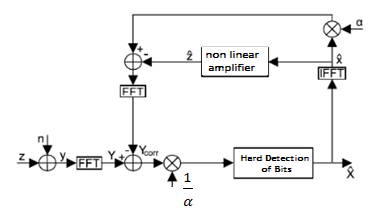
\includegraphics[width=3.5in]{ICDH.png}
\caption{Esquemático do ICHD}
\label{ICHD}
\end{figure}

\subsection{Desempenho da Estrutura}

A Figura \ref{fig:TD} mostra a degradação total considerando-se uma BER de $10^{-3}$. Para o OFDM e o UFMC, a modulação 16-QAM foi considerada, e para o FBMC, a 16-OQAM. Em todos os sistamas, 1024 subportadoras foram usadas, em que 600 carregavam dados efetivamente, enquanto as restantes eram nulas, servindo como banda de guarda. 

Na figura \ref{fig:TD}, nota-se que o UFMC tem um desempenho melhor em termos de degradação total tanto em comparação ao FBMC quanto ao OFDM, os quais, por sua vez, apresentam desempenho bastante similar.Isso sugere que o UFMC é menos afeteado pela amplificação não-linear.

\begin{figure}[h!]
\centering
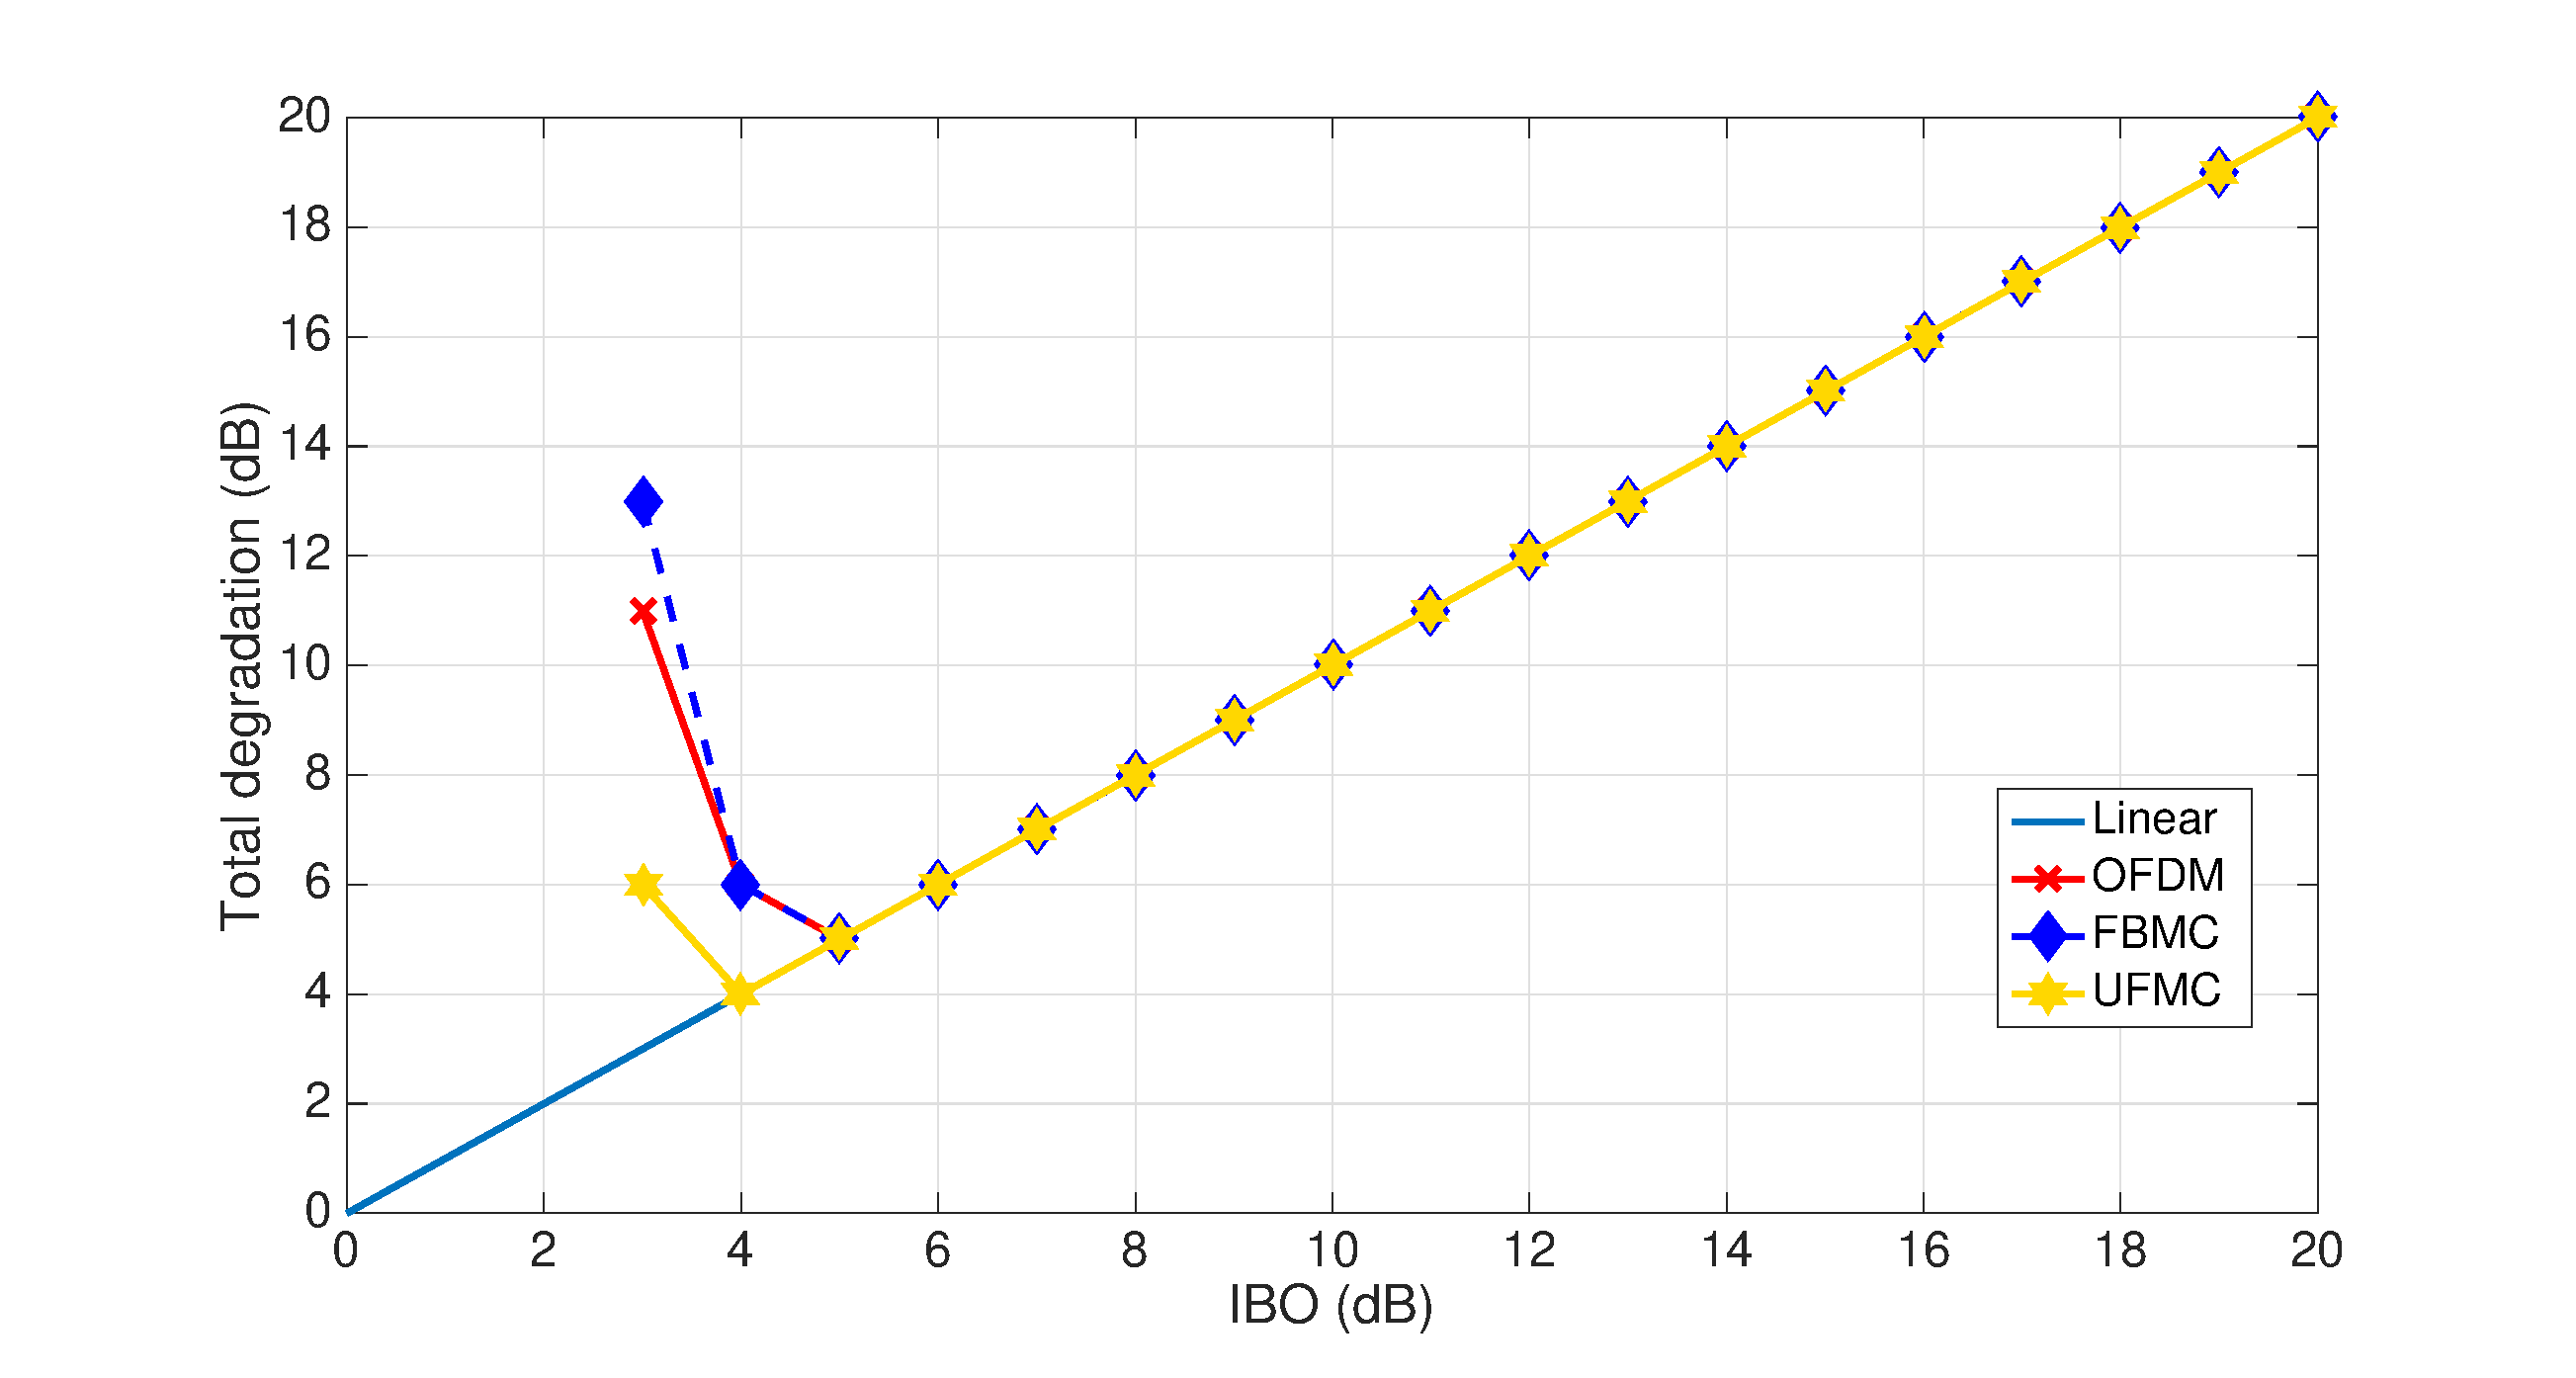
\includegraphics[width=3.5in]{Total_degradation}
\caption{Degradação Total}
\label{fig:TD}
\end{figure}

Como uma referência, o desempenho das três formas de onda aqui investigadas sob os efeitos da amplicação não-linear é apresentado na Figura \ref{fig:linear}. 


\begin{figure}[h!]
\centering
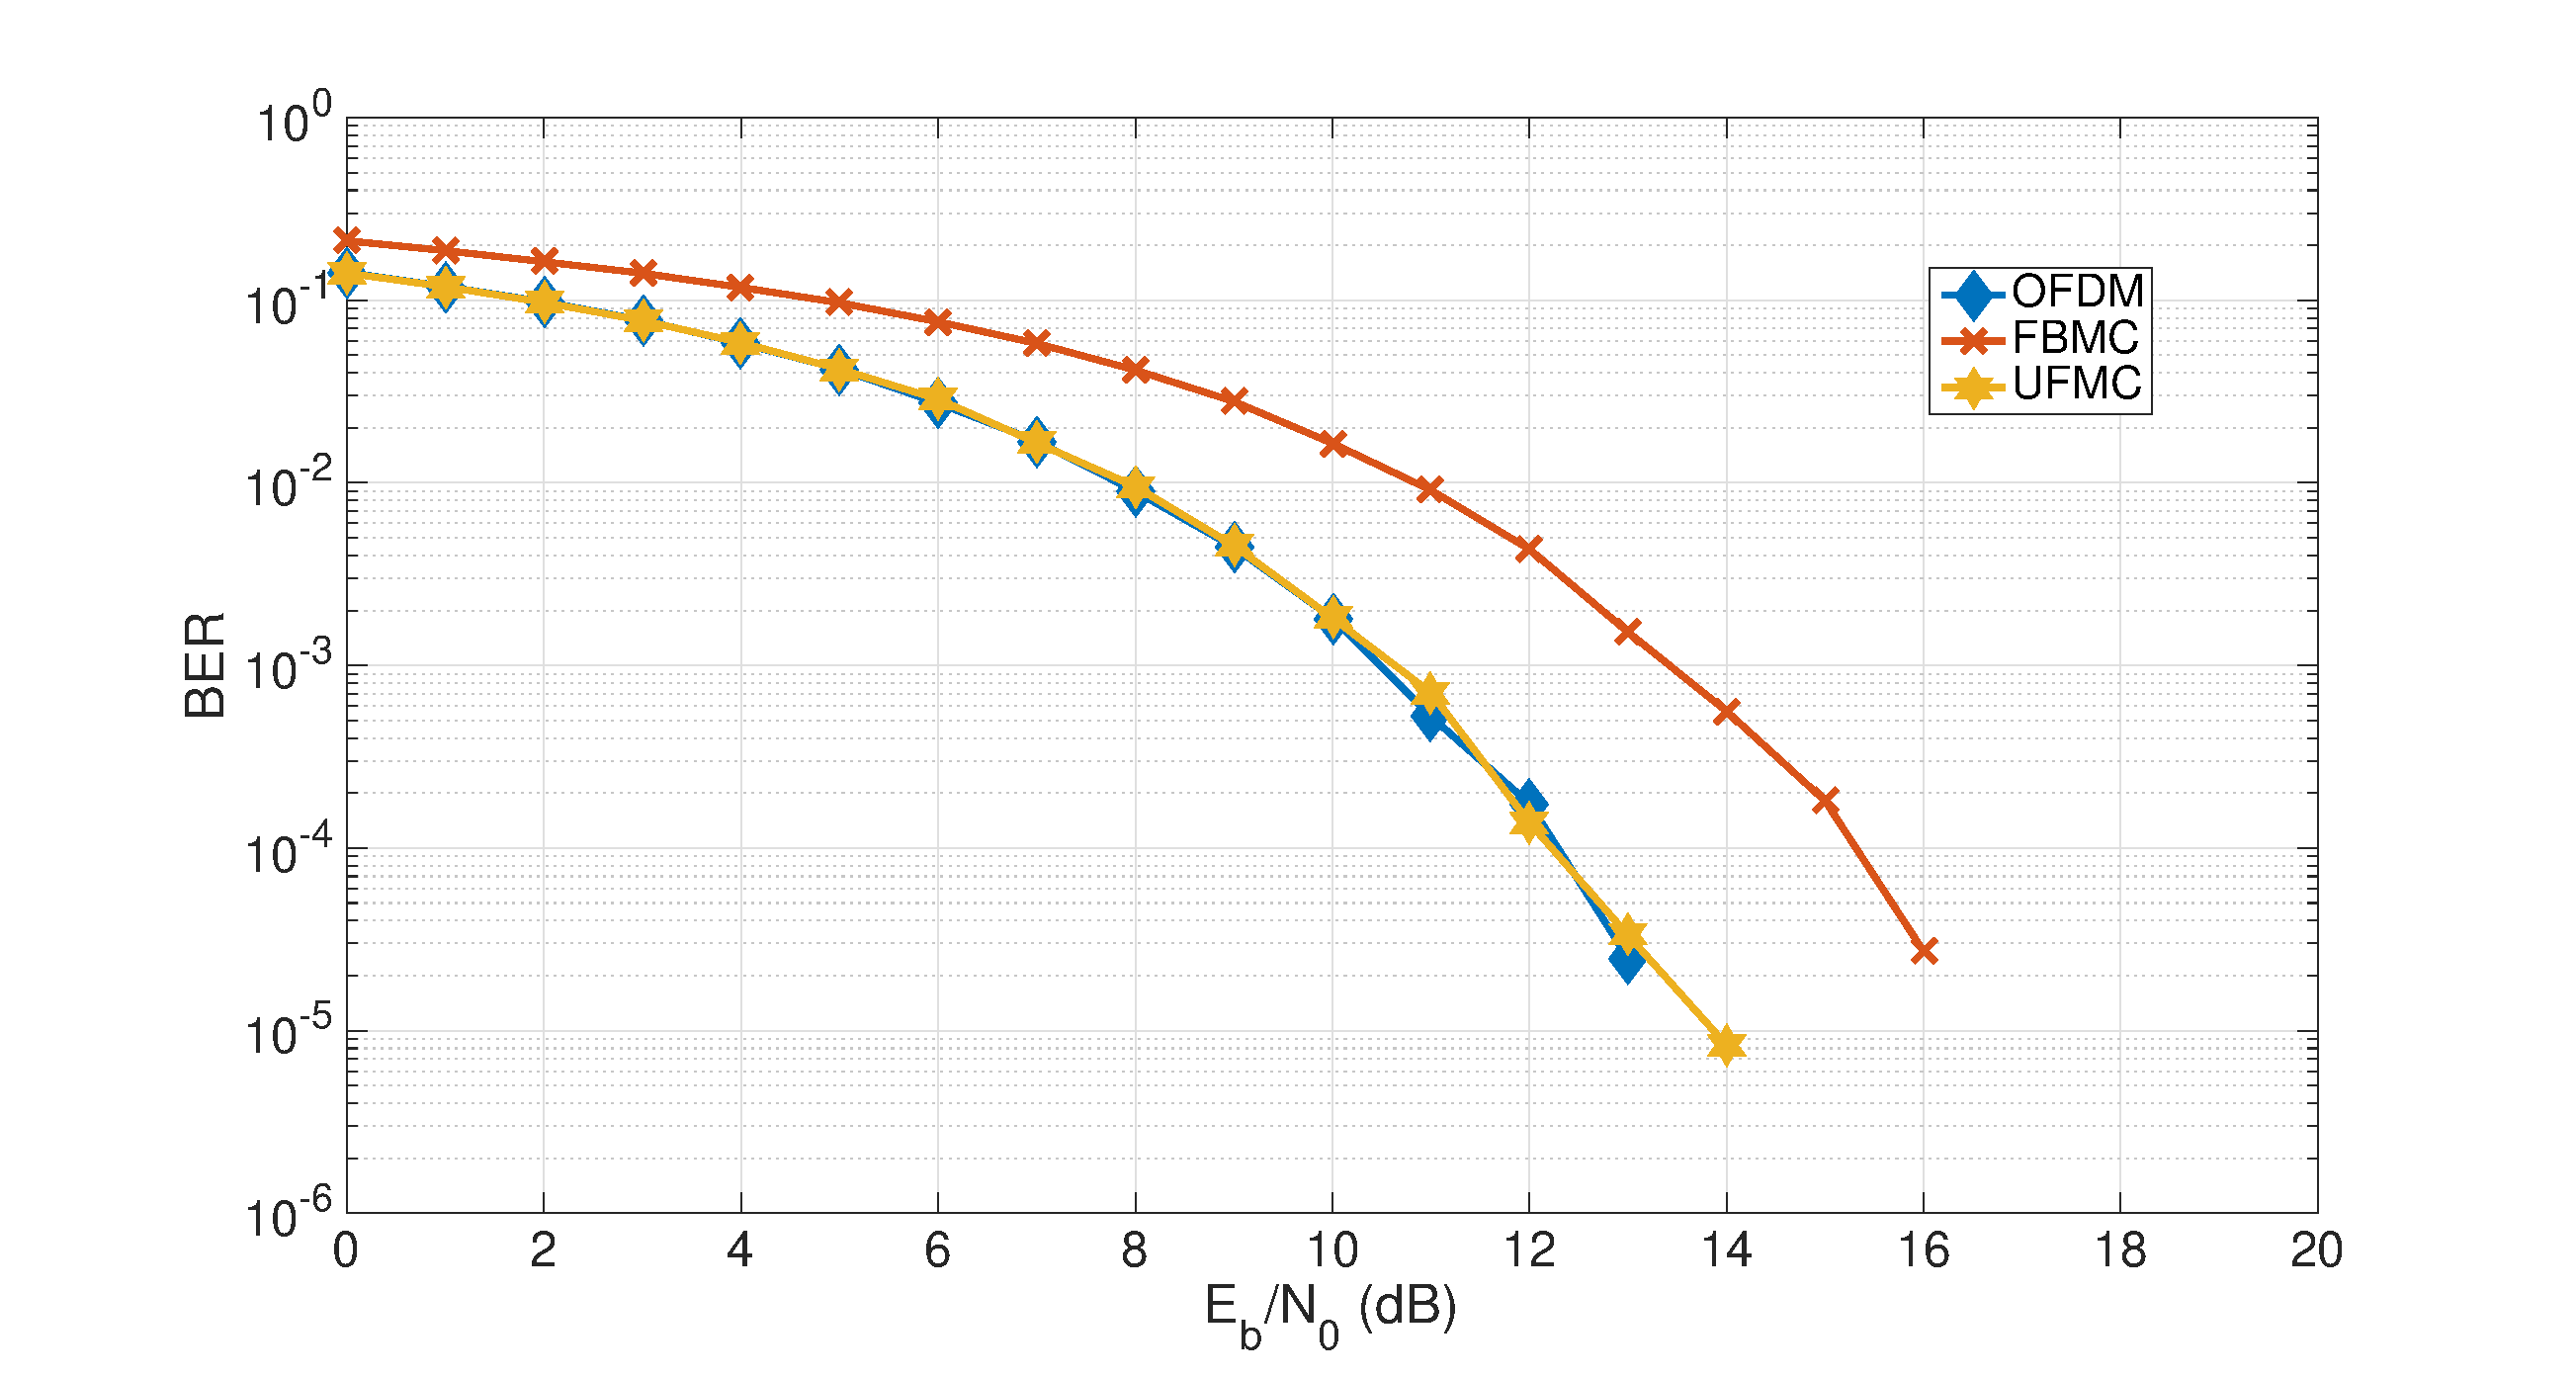
\includegraphics[width=3.5in]{BER_Lin}
\caption{BER para um sistema linear}
\label{fig:linear}
\end{figure}

Nas Figuras \ref{fig:ofdm_ichd}, \ref{fig:fbmc_ichd} e \ref{fig:ufmc_ichd} investiga-se o desempenho do algortimo ICHD algorithm com o OFDM, FBMC e UFMC, respectivamente. Um canal AWGN é usado e nenhum código de correção de erro é aplicado. Ainda, um IBO igual a 3~dB é considerado. Pode-se ver que em todas as figuras, a distorção não linear tem um impacto negativo significativo na taxa de erros. Contudo, também se observa que o algortimo de ICHD algorithm pode melhorar substancialmente o desempenho em termos de BER com apenas algumas iterações, trazendo a resposta próxima ao que se observa em um sistema linear.

\begin{figure}[h!]
\centering
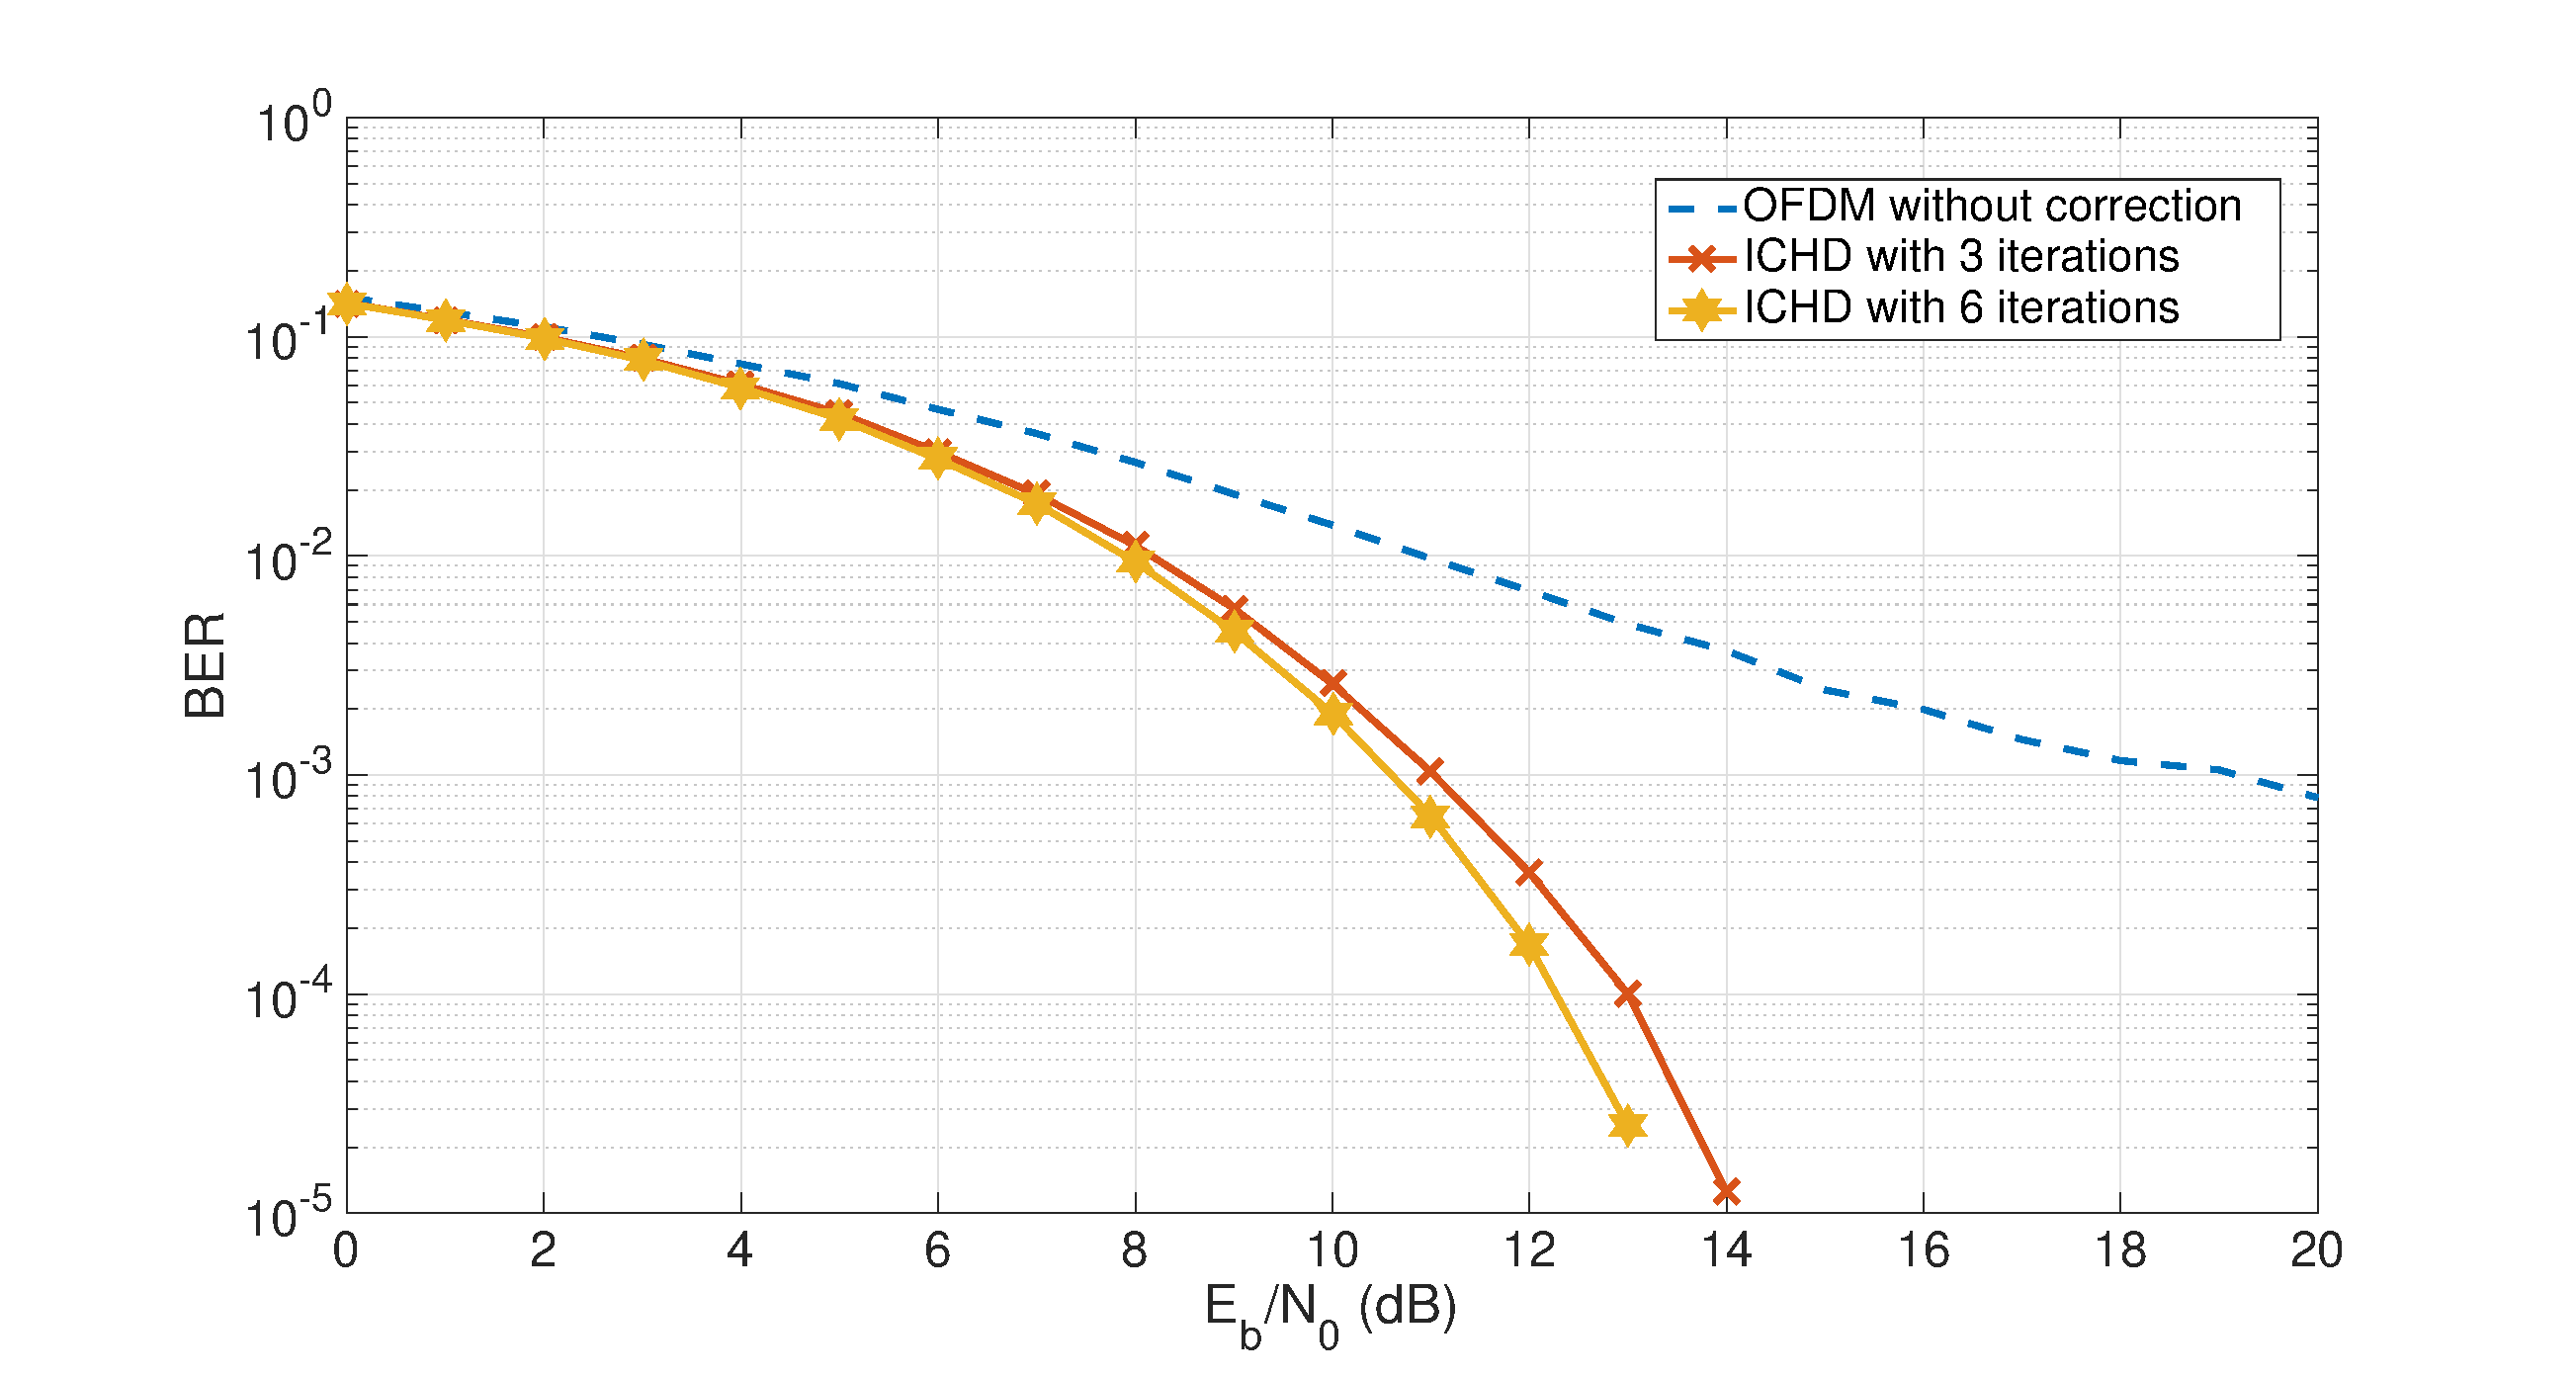
\includegraphics[width=3.5in]{OFDM_ICHD} 
\caption{OFDM com ICHD.}
\label{fig:ofdm_ichd}
\end{figure}


\begin{figure}[h!]
\centering
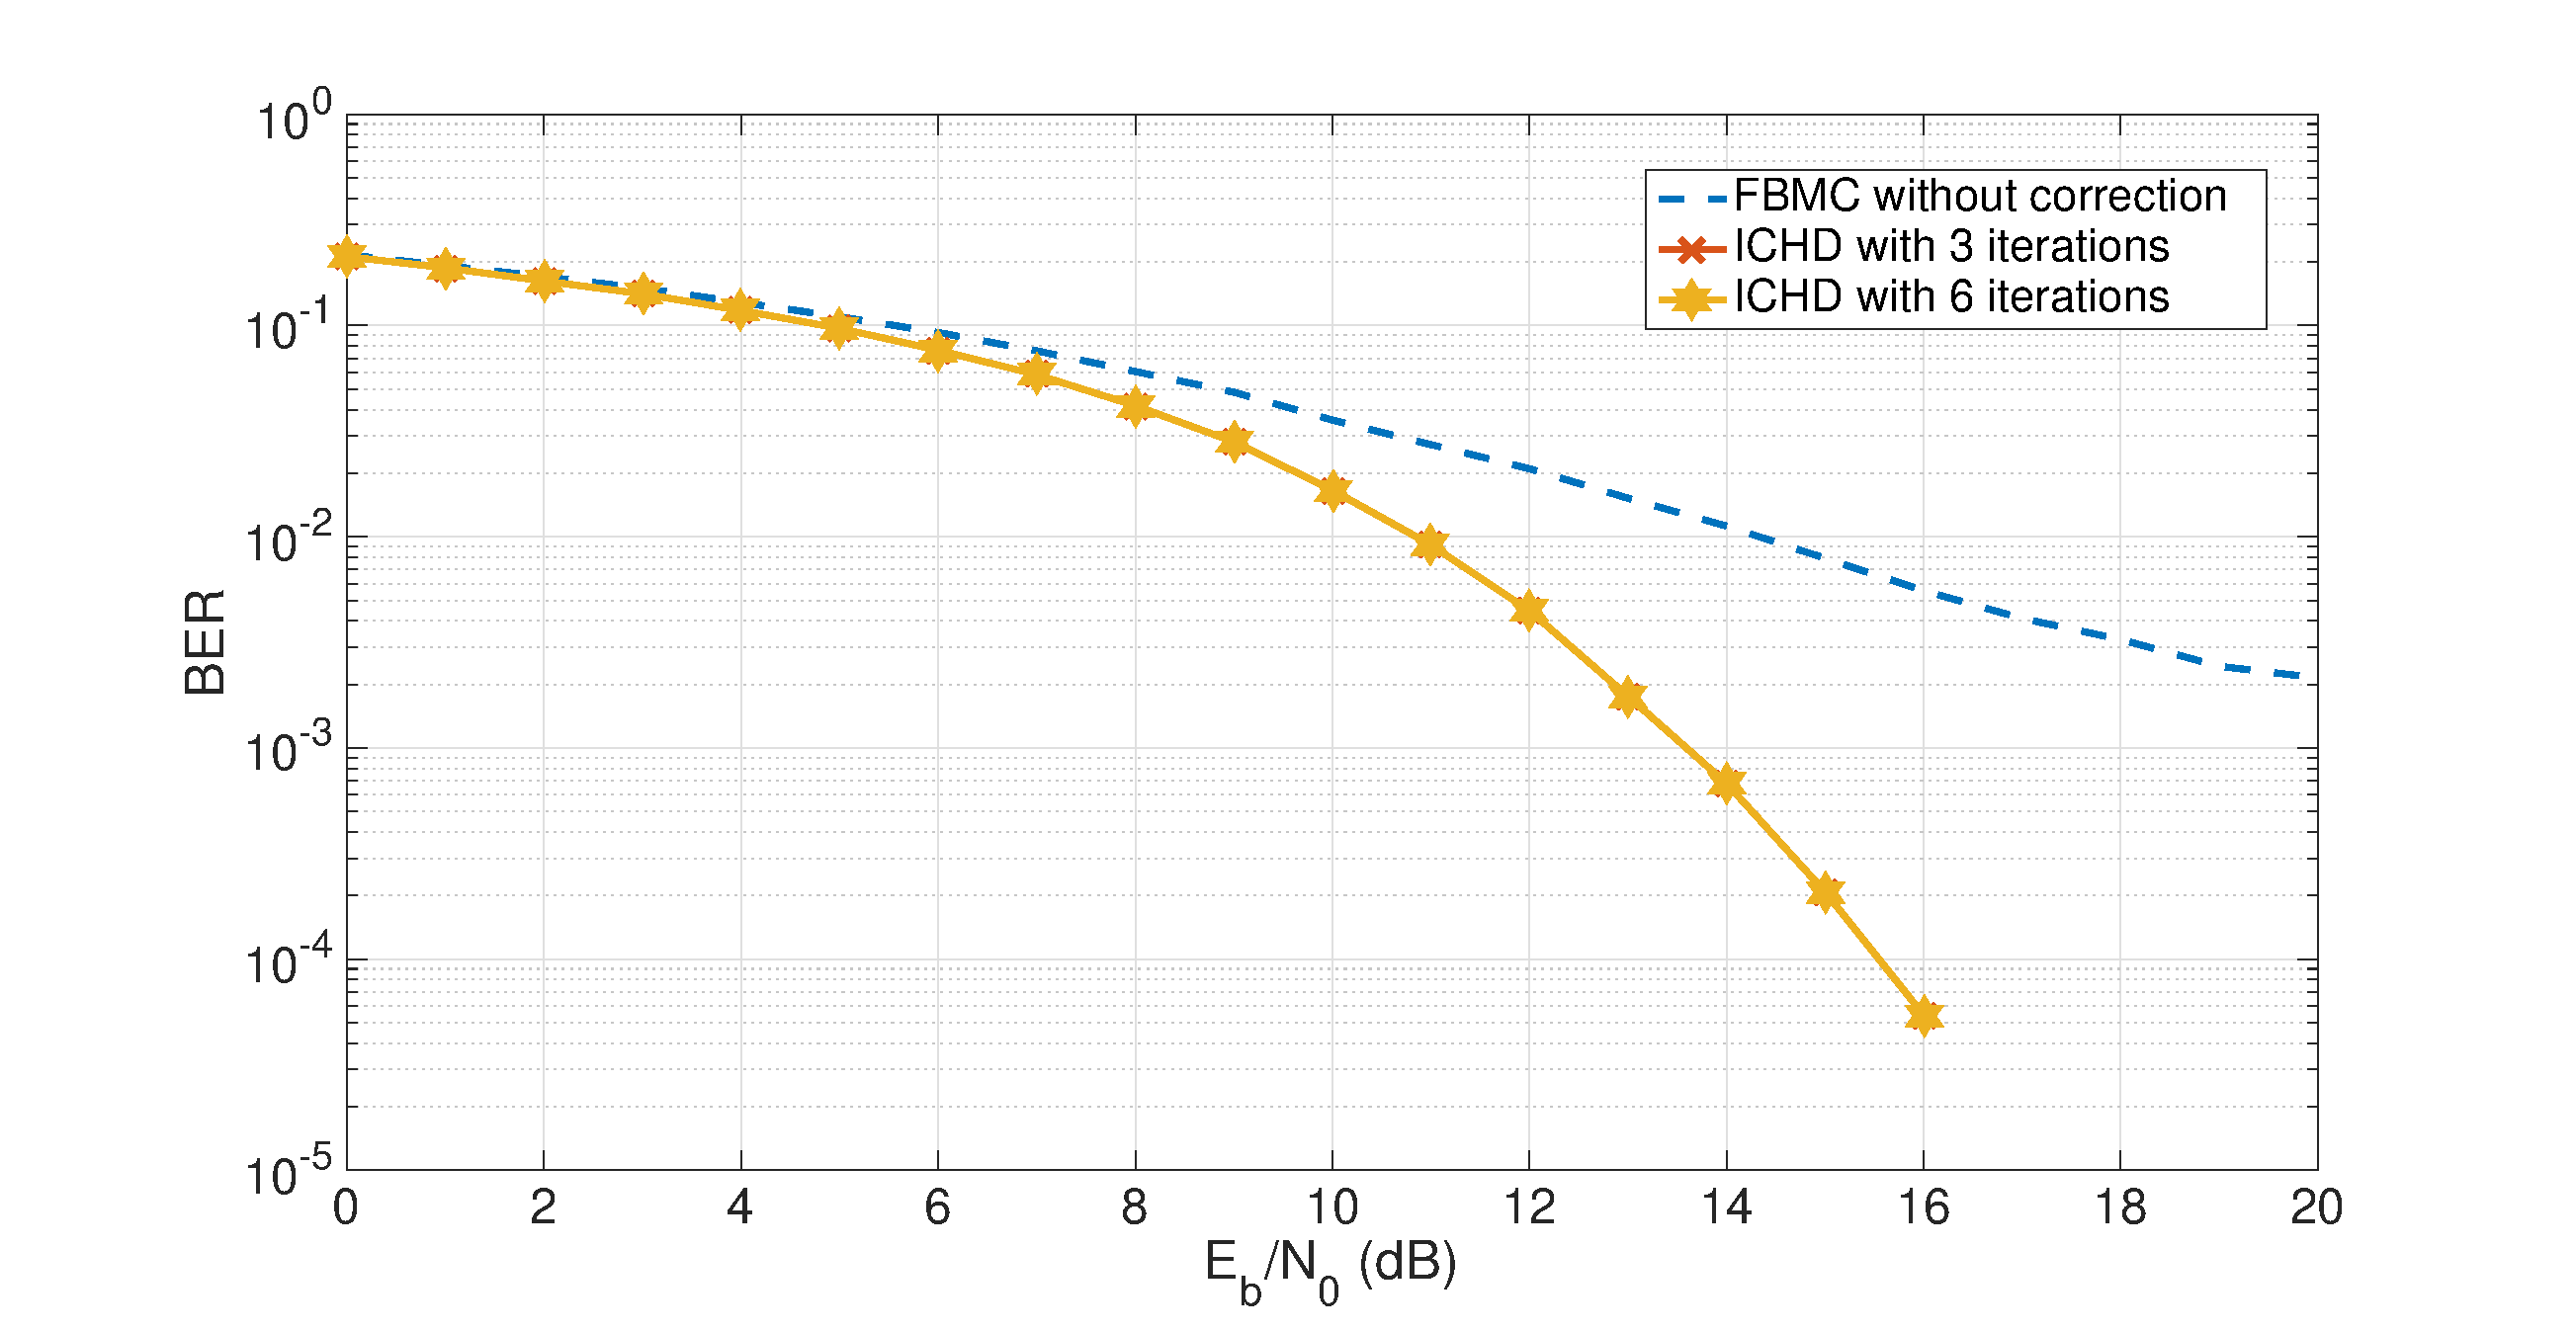
\includegraphics[width=3.5in]{FBMC_ICHD} 
\caption{FBMC com ICHD.}
\label{fig:fbmc_ichd}
\end{figure}


\onehalfspacing
\begin{figure} [h!]
\centering
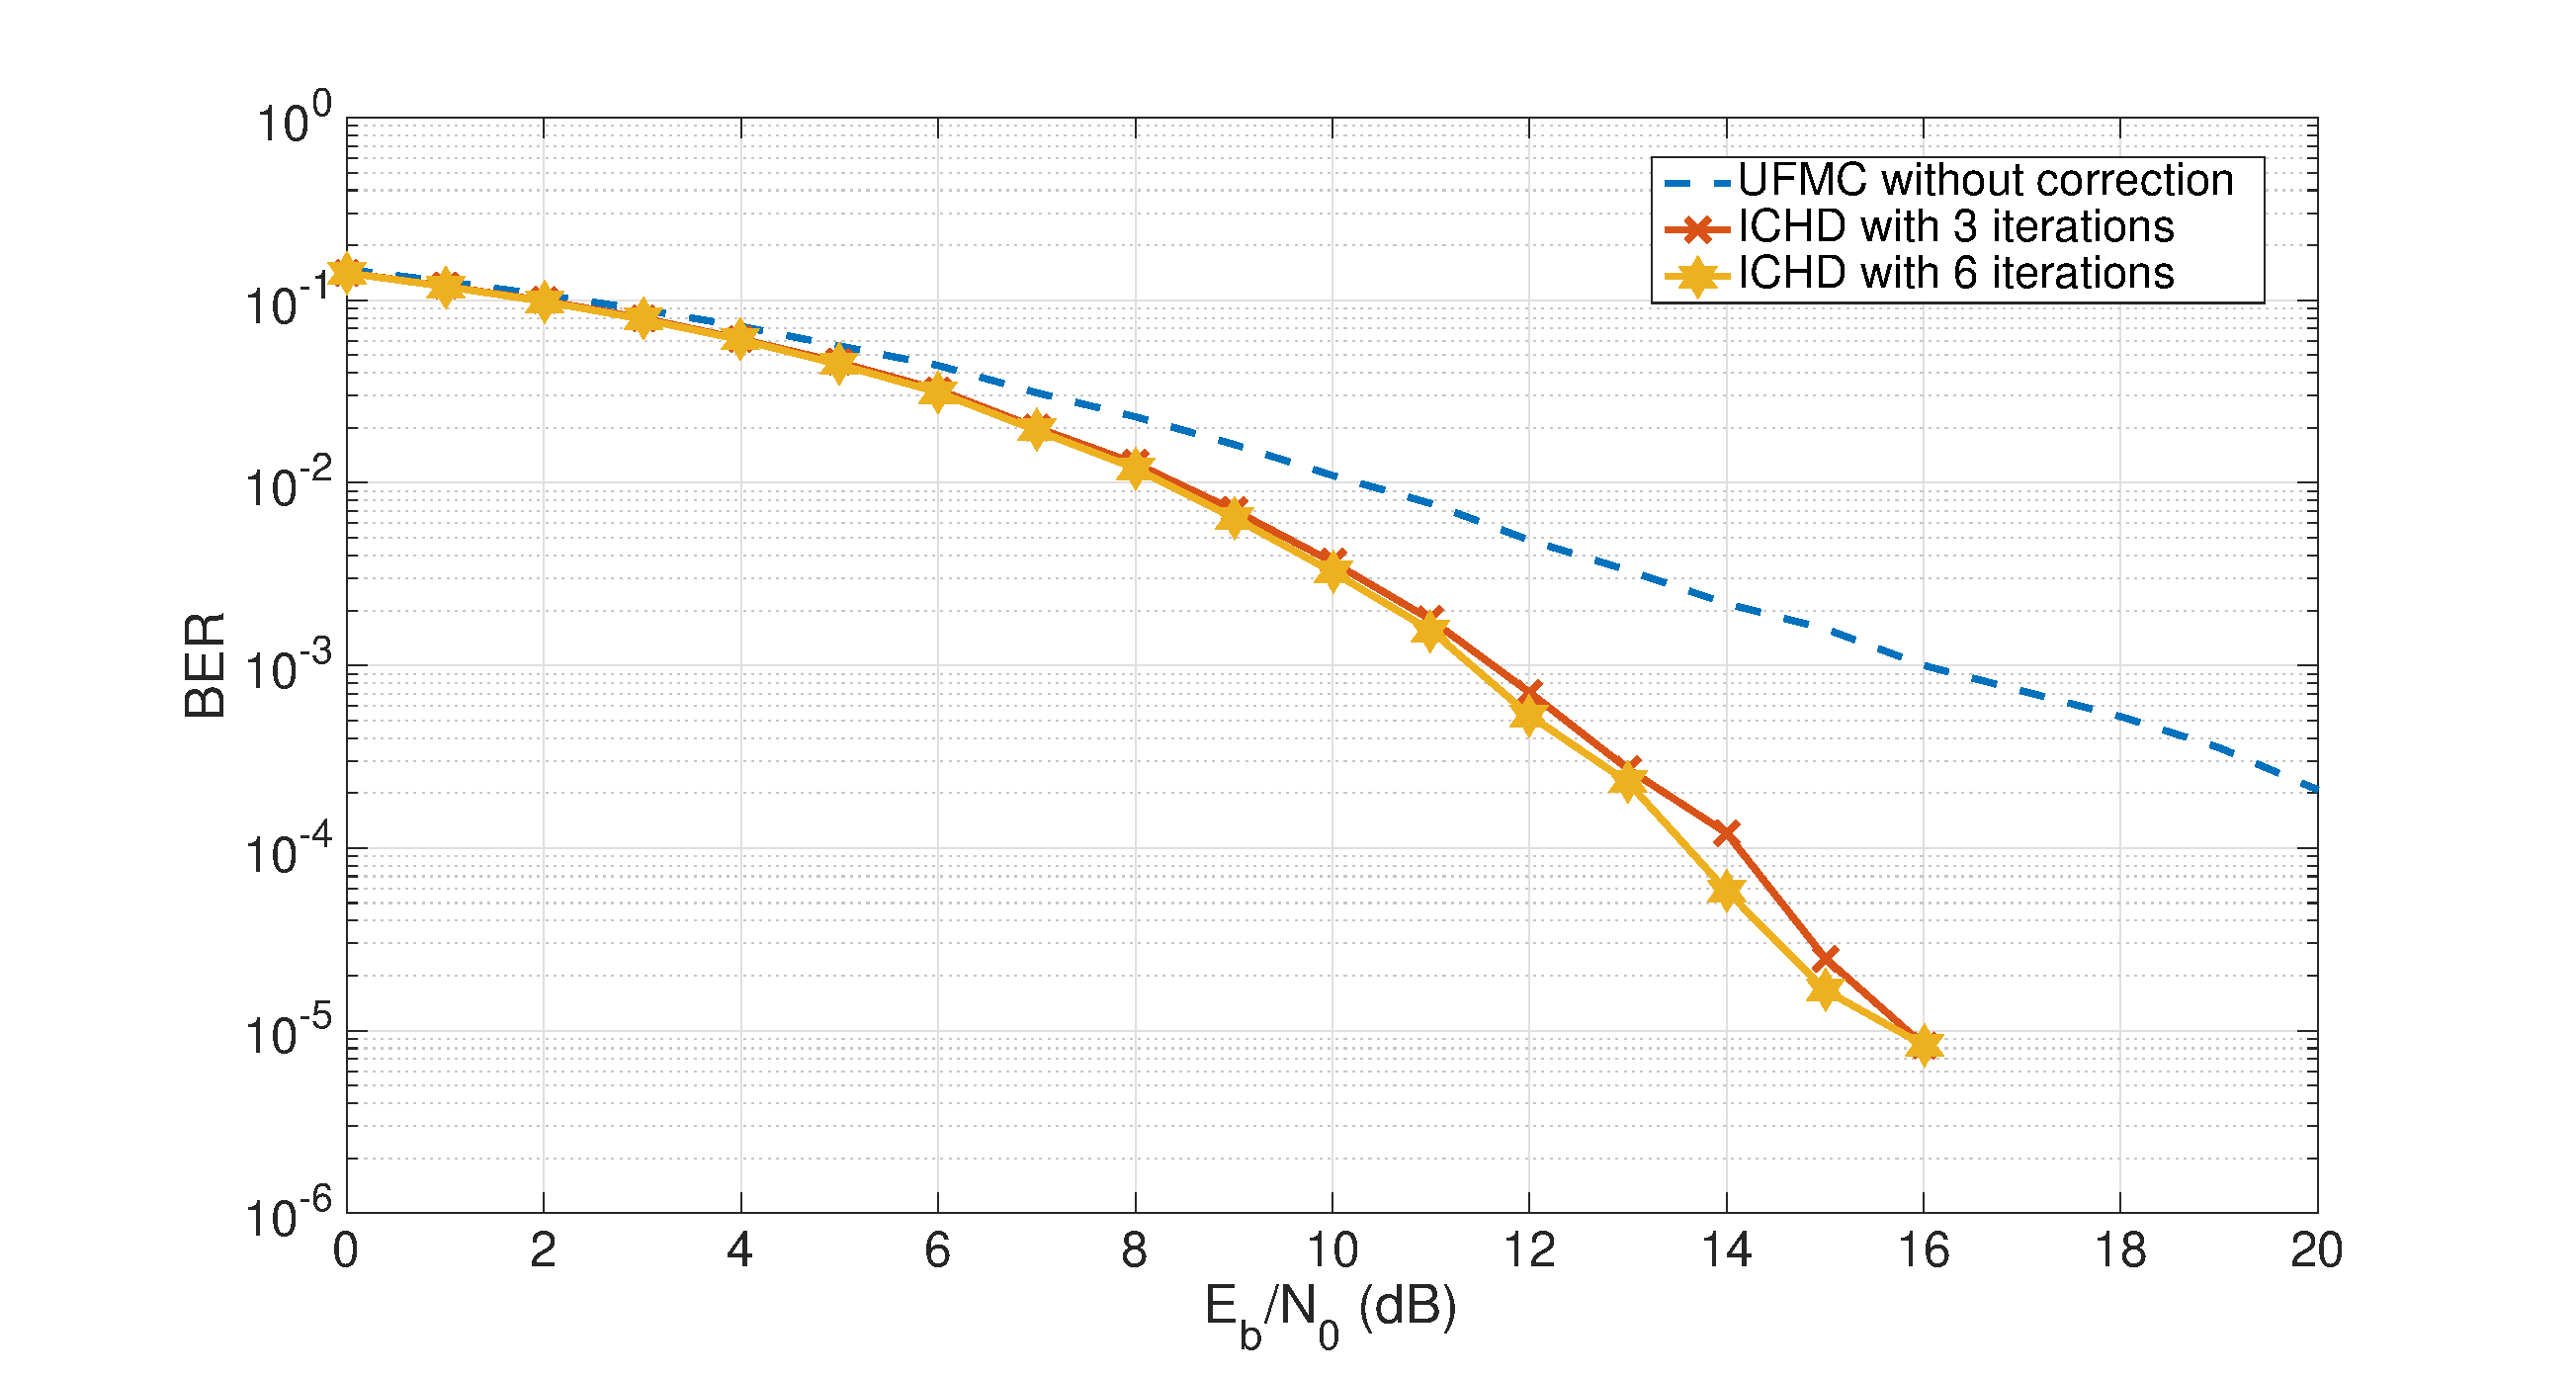
\includegraphics[width=3.5in]{UFMC_ICHD} 
\caption{UFMC com ICHD.}
\label{fig:ufmc_ichd}
\end{figure}

\section{Algoritmo DPD}
Amplificadores de potência devem ser tão eficientes quanto seja possível. Sinais de banda larga, tais como os utilizados em sistemas LTE e aqueles planejados para a 5G, apresentam-se como um grande desagio ao \textit{design} eficiente destes dispositivos, devido aos altos níveis de PAPR, que obrigam a operação dos PA em compressão ou saturação, levando a distroção. \cite{Wood}.  

A possibilidade de utilização de PAs lineares é bastante limitada, então a ideia é lineariazar a entrada do amplificador não lienar. Isto tem se tornado uma técnica amplamente utilizada, deste os anos 1980 para sinais analógicos \cite{Katz} e tornou-se mais comum para esquemas digitais nos anos 1990 \cite{Wood}. Quando aplicada digitalmente, recebe o nome de \text{digital predistortion} (DPD) - predistorção digital.

A técnica de DPD consiste em cancelar a distorção causada por efeitos térmicos e pela própria circuitaria em um sinal de entrada digital que esteja passando através de um amplificador de potência \cite{Dardaillon}. O DPD pode ser dividido em dois passos: estimação e correção.

Estimação é o processo de encontrar uma expressão matemática que represente o comportamento do amplificador. Com os coeficientes estimados em mãos, é possível seguir para o passo de correção. O polinômio estimado é, então, invertido e o sinal de entrada é passado através de um bloco de inversão antes de ser amplificado. 
Os procedimentos são ilustrados pela Figura \ref{FigDPD}, adaptada de \cite{Morgan2006}.

\begin{figure}[h!]
\centering
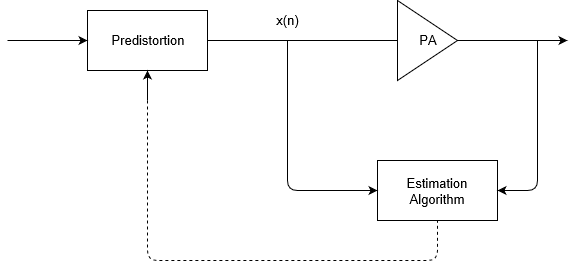
\includegraphics[width=3.5in]{DPDA.png}
\caption{Estrutura DPD}
\label{FigDPD}
\end{figure} 

Comecemos com a estimação:

Este passo é realizado através de um algoritmo de detecção de quadrados mínimos (MMSE) como em \cite{Morgan2006}. Os coeficientes do polinômio da equação \ref{oddpoly} devem ser alinhados em um vetor Jx1, $w$. Fazendo-se isso, o amplificador pode ser expresso por\cite{Morgan2006}:

\begin{equation} 
\label{ampvecq}
\boldmath{\hat{y}} = \boldmath{Xw} 
\end{equation}

em que {$X$} é uma matriz que coleciona as versões atuais e atrasadas de x, em acordo com a equação (\ref{oddpoly}). 

Como a predistroção utiliza a saída $\hat{y}$ em seus cálculos, $\hat{x}$ é a variável de interesse: 

\begin{equation} 
\label{ampvecout}
\boldmath{\hat{x}} = \boldmath{Yw} 
\end{equation}

O erro entre $x$ e $\hat{x}$ deve ser minimizado de tal forma que a estimação esteja próxima a perfeição. Para alcançar isto: 

\begin{equation} 
\label{coef}
\boldmath{w} = \boldmath{(Y^{H}Y)^{-1}Y^{H}x} 
\end{equation}

Em que $Y^{H}$ é a matriz Hermitiana de $Y$. 

Em posse de todos os sistemas utilizados na análise, é possível sequir para a próxima subseção, em que os resultados obtidos através de simulações são apresentados. 

\subsection{Desempeho da Estrutura}

A Figura \ref{fig:non_lin} mostra a taxa de erro de bits para amplificação quando os efeitos de memória são levados em conta. Para as formas de onda OFDM e UFMC, a modulação 16-QAM foi utilizada. Para o FBMC, 16-OQAM. Em todos os sistemas, 2048 suportadoras foram usadas, das quais 1650 carregavam dados, enquanto as restantes eram nulas, servindo de banda de guarda. 

\begin{figure}[h!]
\centering
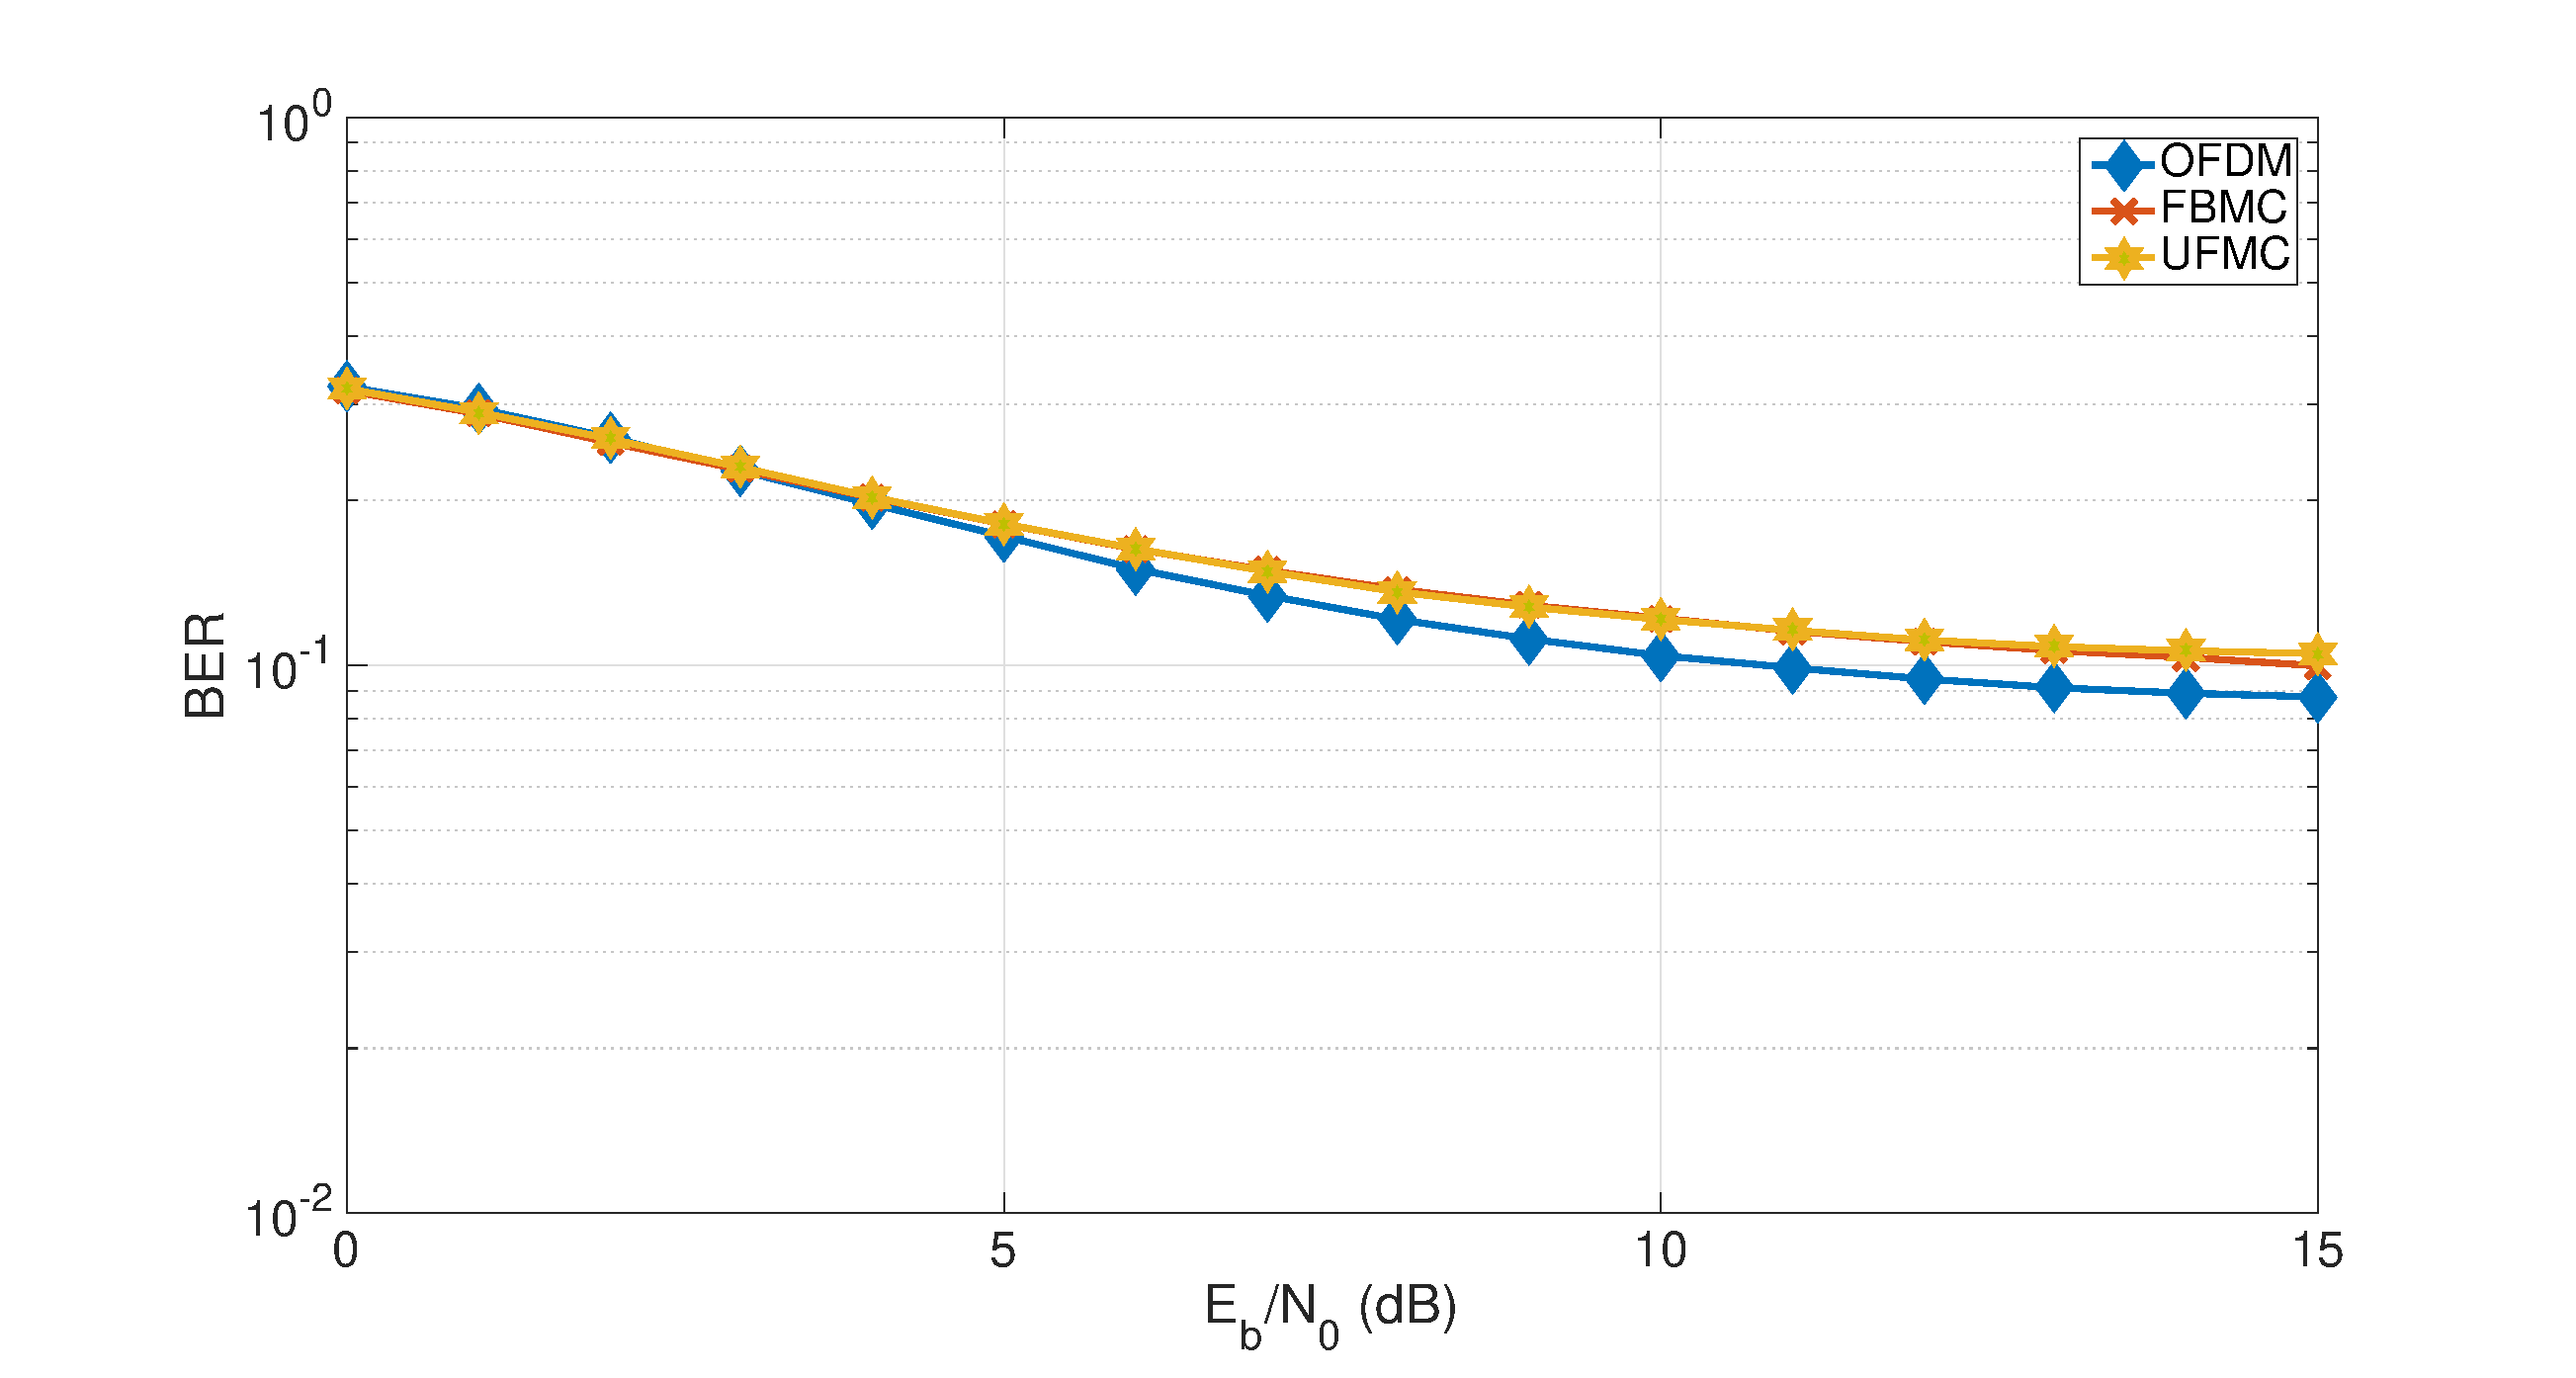
\includegraphics[width=3.5in]{mem_HPA} 
\caption{BER com Amplificadores com Memória}
\label{fig:non_lin}
\end{figure}
A Figura \ref{fig:BER_DPD} utiliza os mesmos parâmetros que a Figura \ref{fig:non_lin}, porém emprega o DPD para linearizar a entrada do amplificador. É possível ver que o DPD funciona de maneira mais efetiva para o FBMC e para o UFMC, os quais superaram o desempenho do OFDM.

\begin{figure}[h!]
\centering
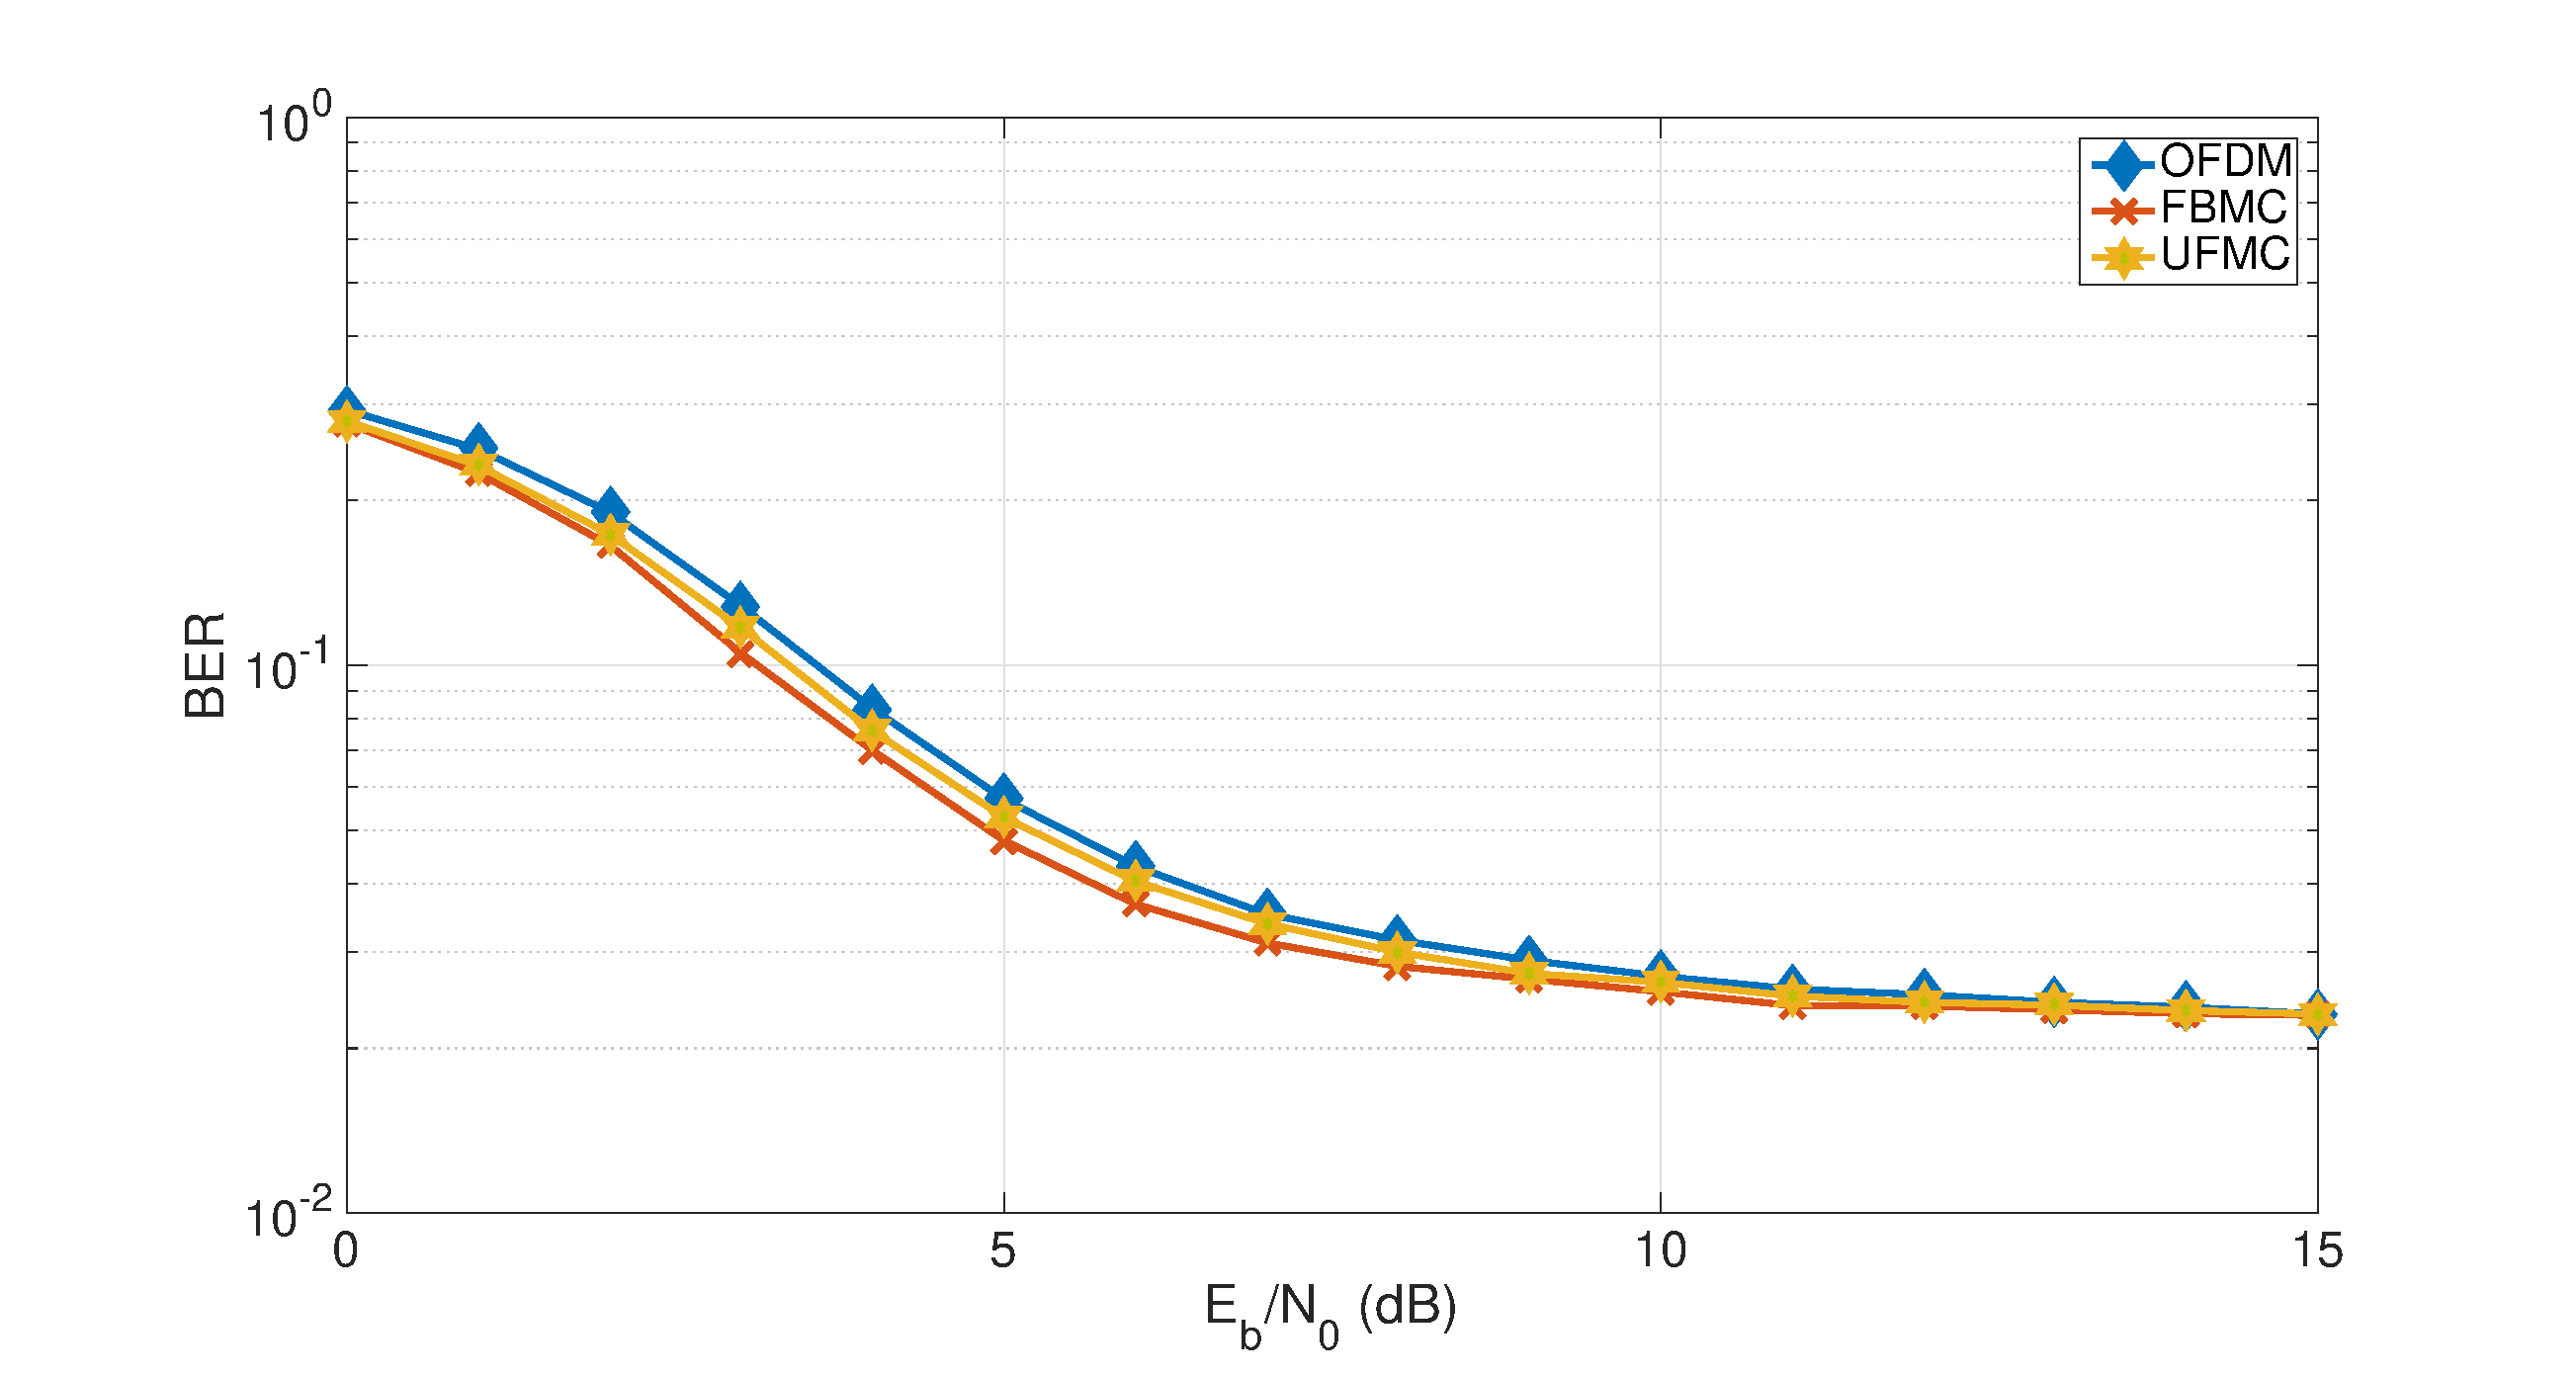
\includegraphics[width=3.5in]{ber_DPD} 
\caption{BER com DPD}
\label{fig:BER_DPD}
\end{figure}

Isso é explicado porque o DPD reduz o espalhamento espectral. Como o FBMC e o UFMC já possuem menos alargamento que o OFDM, um algoritmo que reduz este problema ainda mais melhora o desempenho consideravelmente.

\section{Desempenho com Codificação}